\documentclass[final,5p,12pt,twocolumn]{elsaarticle}
\include{mypackages}
%% \usepackage[
%% backend=biber,
%% style=alphabetic,
%% ]{biblatex}
\newlength{\bibitemsep}\setlength{\bibitemsep}{.4\baselineskip plus .05\baselineskip minus .05\baselineskip}
\newlength{\bibparskip}\setlength{\bibparskip}{0pt}
\let\oldthebibliography\thebibliography
\renewcommand\thebibliography[1]{%
  \oldthebibliography{#1}%
  \setlength{\parskip}{\bibitemsep}%
  \setlength{\itemsep}{\bibparskip}%
}
\usepackage{parskip}
\setlength{\parskip}{10pt} % 1ex plus 0.5ex minus 0.2ex}
\setlength{\parindent}{30pt}
\captionsetup{font=small} 
\begin{document}
\newcolumntype{Y}{>{\small\centering\arraybackslash}X}
\pagenumbering{roman}
\maketitle
\clearpage
%% \title{Comprehensive analysis of electronic noise and their noise spectra of zener diode}
%% \author{Vijay Panchal}
%% \author{Ved Rudani}
%% \address{Department of Physics, Electronics and Space Sciences, Gujarat University, Ahmedabad, India}


\onecolumn
\begin{table*}[hbt!]\centering
  \vskip50pt
  \parbox[h]{.75\textwidth}{\centering \hrule height 2pt \vskip10pt\Large \textbf{Abstract} \vskip10pt \hrule height 2pt \vskip10pt}
  \parbox[h]{.75\textwidth}{\normalsize \textbf{
       Abstra fasdfslkaf sfskjsalk flkasjddfklja slfkjakslfjlkajsfkl asjfkjakfjkjfkl 
} \vskip10pt \hrule height 2pt \vskip10pt}
\end{table*}
\clearpage
\begin{table*}[hbt!]\centering
\vskip20pt
\parbox[h]{.75\textwidth}{\tableofcontents}
\end{table*}
\clearpage
\twocolumn

\pagenumbering{arabic}
\section{Introduction}\label{introduction}
%% \vspace{-2mm}
This is our master’s semester four project report. We have done work on instrumentation for finding magnetic susceptibility of unknown samples. Our final goal is to find phase transitions of samples under change of temperature. We got needed help from the department of physics’s condensed matter laboratory, Dr. Utpal Joshi, Swati Pachauri. Lock-In amplifier that we got access from Utpal sir and it  was a necessary component in our project. 

In this project we did first to design and improvise our instrument, which is an AC susceptometer. Major problem faced by such a setup by non-expert is the problem of noise. We gave our best time for this to get as minimum noise as possible. This was a very big task for us. Another thing which made us think is that of getting offset null for AC susceptometer. We did this by changing the coil's parameter and relative orientation of the coils with each other. Final giant in our project was calibration, as it turns out our instrumentation has some noise floor and for samples, especially that of paramagnetic, have very feeble magnetization which is hard to detect with our setup. So, we choose ferromagnetic samples such as nickel, LSMO and $Gd_2O_3$. Problem with these samples was that their magnetic susceptibility is highly dependent on conditions of measurement, so we can’t find its absolute values like paramagnetic samples. This problem seems to be big for calibration of our instrument. Finally we have tried and successfully calibrated with some accuracy. Final goal was to find temperature dependent magnetic susceptibility plots and find curie temperature where magnetic phase transition happens. This task does not need very accurate calibration and is possible with our instrumentation.

%% \section{Theoritical concepts}\label{theory}
%% \subsection{Magnetism}
We should know little about some concepts of magnetism. Magnetism in loops is profoundly due to relative motions of charge particles. This is related to concepts of relativity (especially Einstein’s special relativity). As we know moving charge creates a magnetic field which curls around movement direction. These magnetic fields get accumulated with a number of loops which relate to our instrumentations. Also, changing velocity (relates directly to changing current) creates a changing magnetic field.

There’s another type of magnetism which differs in some minor differences. This is related to the material’s magnetic moments. As we know atoms have magnetic moments related with two momentums,orbital angular momentum and spin angular momentum. This degrees of freedom of electrons (as by product relates to atoms) creates magnetic properties of materials. 

%% \subsection{Spins}
First evident by Stern and Gerlach 

A magnetic susceptibility of a material can be defined as the amount of a material gets magnetised , when it is placed in an external magnetic field .
In other words , an amount of magnetization of a material occurs when it is placed in external magnetic field .

An expression for magnetic susceptibility is given by ,

                  Χ = M / H

Where , M= Magnetic susceptibility 
              H= Applied/External magnetic field 

There are two other measures of susceptibility:

1. MAGNETIC MOLAR SUSCEPTIBILITY (Χm)

2. MASS MAGNETIC SUSCEPTIBILITY (Χр)

                   Χm = M Χр

Where,  Χр= Χv / р , р= density (kg/m^3)

Magnetic susceptibility is a factor that indicates the magnetic behavior of a material.It gives an idea about a material that it can be attracted or can be repelled. 


CLASSIFICATION OF MATERIALS BASED ON THEIR MAGNETIC PROPERTIES :-

DIAMAGNETIC MATERIAL :

A magnetic materials which aligns its domains or field lines against the applied magnetic field are known as diamagnetic materials.

These materials are strongly repelled by the magnets .

As these materials gets magnetize in opposite side of applied field , they have a small amount of magnetization .

Example :- water, tin , mercury ,etc.

They have magnetic susceptibility Χ < 0,
negative value of magnetic 
susceptibility.

          2 .  PARAMAGNETIC MATERIAL :

A magnetic materials which aligns its domains or field lines with the applied field are known as paramagnetic materials .

These materials are weakly attracted by the magnets and also they are temperature dependent .

Example :- aluminium , alkaline earth metals , etc.

They have magnetic susceptibility Χ > 0 , positive value of magnetic 
susceptibility.

            3 .  FERROMAGNETIC MATERIAL :

A magnetic materials that are highly gets magnetized in an external magnetic field are known as ferromagnetic materials .

These materials are highly attracted by the magnets .

Example :- iron, cobalt, nickel , etc .

They have magnetic susceptibility Χ > 1, always higher value of magnetic susceptibility.
 
There are further classification of materials based on their magnetic properties can be done as :

a) Anti-ferromagnetic materials 

b) Ferrimagnetic materials 

These two types are not discussed in detail because they are not in context to our project work .

WHAT DO YOU MEAN BY AN AC MAGNETIC SUSCEPTIBILITY ?

AC magnetic measurements are taken by applying AC field to the samples and resulting AC magnetic moment is measured i.e.,
induced by changing magnetic flux by applied AC field .

This results in the different values of magnetic susceptibility for different values of magnetic flux arises from the different values of AC field.

In order to understand AC magnetic susceptibility , first we have consider measurements at low frequencies , where the 
measurements is almost equals to the DC susceptibility.In this case the absolute value of magnetization is calculated i.e.,

 Χ = M / H

In case of AC susceptibility, the continuously varying value of magnetization , hence varying value of susceptibility i.e.,

 Χac = (dM / dH)

AC susceptibility is often referred as dynamic susceptibility.AC measurements are very sensitive to the small changes in the values of magnetization .


\section{Experimental setup}\label{setup}
Setup was done in such a way that approximately all the instrument's magnetic field cancels out; only remaining is that of sample’s magnetization.  This can be done by canceling mutual inductance of measuring coils. 
\subsection{Coil assembly}
Coils in Setup have two types. One is the primary coil which produces a magnetic field. Second is that of secondary coils which couple with primary and produce mutual inductance. Primary coil is connected to the input signal which is nothing but a reference signal from the LOCK-IN amplifier. This creates a changing magnetic field. 

%% \begin{figure*}[hbt!]
%%   \centering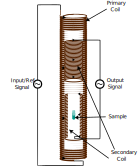
\includegraphics[width=0.8\textwidth]{coils.png}
%%   \caption{This is the main setup of the experiment. you can see primary coil and two secondary coil winded opposite directions}
%%   \label{fig:assembly}
%% \end{figure*}

This changing magnetic field is picked up by secondary coils which generate inductive current, but they are winded in the opposite direction. Thus, their current cancels out resulting in zero output signal. When sample is in anyone of these coils, generates some residual magnetization and resultant signal. This signal $V_{out}$ is proportional to $\chi$ of the sample. Geometry of coil is given in table 1. Also, figure \ref{fig:assembly} shows the coil assembly of our setup.

\noindent\setlength\tabcolsep{4pt}%
\begin{tabularx}{\linewidth}{|c|Y|c|Y|c|Y}
  \hline
  \hline
  & Primary Coil & Secondary Coil \\
  \hline
 Diameter of wire & 30 gauge & 38 gauge \\
 Length of winding & 20 cm & (8.3 + 8.3) cm \\
 No. turns & 550 & (450 + 450)\footnote{symmetrical winding, 450 clockwise and 450 anticlockwise}\\
 \hline
 \hline
 \caption{Geometry of coils in our setup}
 \label{geometry}
\end{tabularx}

\begin{figure*}[h]
  \centering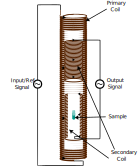
\includegraphics[width=0.7\textwidth]{coils.png}
  \caption{This is the main setup of the experiment. you can see primary coil and two secondary coil winded opposite directions}
  \label{fig:assembly}
\end{figure*}



\subsection{Offset Settings}

At the initial stage, we have to offset null between two secondary coils voltage measurement. As a matter of facts we tried to take both our coils to be as symmetrical as possible but inherent human error is there. For this issue we took certain steps,

  
\begin{itemize}
\item Very crudely we take out windings or wind up. This is to balance both secondary coils to almost perfection. This method is quite clumsy and pain staking. The offset still remains and we can’t go beyond the noise limit of the instrument.
\vskip1cm
\item Another thing we can do is that of using some external balancing circuit. Since we have very limited time we can’t go down to this rabbit hole.
\end{itemize}
\vskip1cm
Finally we decided to ignore some offset and subtract it from data of background. This way is not that effective but we don’t have other options.


\subsection{Calibration}


The giant task of our project was to calibrate our handmade instrument. This is also benign by noise of instruments and readings. We made a decision and did this the following way. As it turns out, Calibration can be done in two ways.\cite{cambr} 
\vskip1cm
\begin{itemize}
\item Theoretically, by mutual inductance calculation, which can give exact value of how much field inside of sample. \cite{10.1063/1.1137813}
\vskip1cm
\item Experimentally, by taking some standard susceptibility values of some known and reliable sample.
\end{itemize}
\vskip1cm
There is still one catch, what we need is some $\chi_{int}$\cite{cambr}. What we are measuring is $\chi_{ext}$. What are these different values of susceptibilities? Well as it turns out the $\chi_{int}$ is what we expect from theoretically, 


\begin{equation*}
\chi_{int} = \frac{dM}{dH}
\end{equation*}
 And 
\begin{equation*}
\chi_{ext} = \frac{dM}{dH_a}
\end{equation*}
 
This two values are related by following identity \cite{cambr},

\begin{equation*}
\chi_{int} = \frac{\chi_{ext}}{1-D\chi_{ext}}
\end{equation*}

This value $\chi_{ext}$ is what we took proportional in the previous topic as LOCK IN’s output signal $V_{out}$. If we take the first equation then we can approximate the calibration constant to some extent, we took the second way that is experimental. We took some samples that can give out certain values of output. Before going there, we calculated for the first method. Simplified setup for primary coil is shown in figure  \ref{fig:circuit}. Here we neglected the back inductance of the secondary coil.

\begin{figure}
  \includegraphics[width=1\linewidth]{circuit.png}
  \caption{This is a simpler circuit of coil assembly in our setup. we are neglecting effect of second coil}
  \label{fig:circuit}
\end{figure}

Simplified circuit makes following kind of differential equation,

\begin{equation}\label{diff}
  V_{in}-L\frac{dI}{dt}-IR=0
\end{equation}

Where, $V_{in}$ is nothing but $V_{ref}$ from the LOCK IN amplifier.  It is of the following form $V_{in} = V_0 e^{i(w_rt+\phi_r)}$, $w_r$ is applied frequency, $\phi_r$ is taken as zero from input. $I$ is current in the primary, this parameter is very important and gives applied magnetic field strength $H_a$. $L$ and $R$ are both electrical parameters of the primary coil, respectively self-inductance and resistance. Solution of equation \ref{diff} gives current in primary at instance of time,

\begin{equation}
I_{real} = \frac{V_0\left[\frac{R}{L} cos(w_rt+\phi_r)+w_r sin(w_rt+\phi_r)\right]}{L(\frac{R^2}{L^2}+w_r^2)}+Ce^{-\frac{R}{L}t}  
\end{equation}

\begin{equation}
I_{imag}=\frac{\left[\frac{R}{L} sin(w_rt+\phi_r)-w_r cos(w_rt+\phi_r)\right]}{L(\frac{R^2}{L^2}+w_r^2)}
\end{equation}

If we take $\phi_r = 0$ and $V_0 = 1 V$ which signifies that total input phase and amplitude of reference voltage from LOCK IN amplifier is 0 deg and 1 V. Here, $C$ is an integral constant.
 

\begin{equation}
I_{real} = \frac{\frac{R}{L} cos(w_rt)+w_r sin(w_rt)}{L(\frac{R^2}{L^2}+w_r^2)}+Ce^{-\frac{R}{L}t}
\end{equation}

\begin{equation}
I_{imag}=\frac{\frac{R}{L} sin(w_rt)-w_r cos(w_rt)}{L(\frac{R^2}{L^2}+w_r^2)}
\end{equation}

 After taking condition that initial current is zero, 

\begin{equation}
C = \frac{-R}{L^2(\frac{R^2}{L^2}+w_r^2)}
\end{equation}

\begin{equation}
I_{real} = \frac{\frac{R}{L} cos(w_rt)+w_r sin(w_rt) -\frac{R}{L}e^{-\frac{R}{L}t}}{L(\frac{R^2}{L^2}+w_r^2)}
\end{equation}

From this current magnetic field strength inside primary coil and coupled by secondary coil is as following

\begin{equation*}
H_a(t) = c N I(t)
\end{equation*}

Which is measured in $A/m$, here $c$ is coupling constant for secondary coil. Since, the magnetic field inside the coil is not homogeneous, finding this parameter is very difficult, also if we find it then we get averaged out readings for whole coil. Magnetic field inside coil $B=\mu_0 H_a$. Also, flux inside secondary coil is as following, 

\begin{equation*}
\Phi = \mu_0 H_a n \pi a^2
\end{equation*}

Hare, $n$ and $a$ are geometrical parameters of the coil, $n$ is the number of turns of a single secondary coil and $a$ is the diameter of the secondary coil. We took the secondary coil in the centre of the primary coil as possible.
\begin{equation*}
\Phi = M I
\end{equation*}
\begin{equation*}
\frac{d\Phi}{dt} = M \frac{dI}{dt}
\end{equation*}

Here, $M$ is a mutual inductance parameter, which only depends on setup and sample placement. Final, voltage measurement from our secondary coil is only dependent in only LOCK IN readings \cite{cambr},

\begin{equation*}\label{thiseq}
V_{out} = \alpha H_a f V_{sample} \chi_{ext}
\end{equation*}

Here, $\alpha$ is calibration constant, which we have to determine. Theoretically, We know $H_a$, $V_{sample}$ (volume of sample: we took some small cylindrical capsule), $f$, $\chi_{ext}$ then we can find $\alpha$ directly. But knowing this parameter and their exact place in the instrument is very difficult. This is problematic. So, we turn to the second method and fix the orientations and parameters, put some sample and compare its reading calculated by their known magnetic susceptibility. 

For calibration purposes we took four samples and their readings of output voltages. These are 1. $Fe_2O_3$, 2. Nickel, 3. LSMO (Lanthanum strontium manganite), 4. $Gd_2O_3$. For characterization purposes $Fe_2O_3$ and $Gd_2O3$ are paramagnets where Nickel and LSMO are Ferromagnets. Problem we faced in our measurement is that our instrument’s sensitivity is very low and sample weight is very small. As a result paramagnetic substances have feeble signals which are not very reliable compared to ferromagnets like Nickel and LSMO. The data are shown in figures \ref{fig:Rdata1}, \ref{fig:Rdata2}, \ref{fig:Rdata3} and \ref{fig:Rdata4} where you can see why ferromagnets signal is reliable.

\begin{figure}[hbt!]
  \includegraphics[width= \linewidth]{plots/fe2o3R.png}
  \caption{Plot of absolute values of voltage $Fe_2O_3$ and it's Background. You can see difference is $5.212068 \times 10^{-7}$}
  \label{fig:Rdata1}
\end{figure}
\begin{figure}[hbt!]
  \includegraphics[width= \linewidth]{plots/gd2o3R.png}
  \caption{Plot of absolute values of voltage $Gd_2O_3$ and it's Background. You can see difference is $3.543178 \times 10^{-7}$}
  \label{fig:Rdata2}
\end{figure}

Also values for Nickel and LSMO. You can see stark differences.

\begin{figure}[hbt!]
  \includegraphics[width= \linewidth]{plots/LSMOR.png}
  \caption{Plot of absolute values of voltage $LSMO$ and it's Background. You can see difference is $2.257564 \times 10^{-4}$}
  \label{fig:Rdata3}
\end{figure}
\begin{figure}[hbt!]
  \includegraphics[width= \linewidth]{plots/nickelR.png}
  \caption{Plot of absolute values of voltage Nickel and it's Background. You can see difference is $2.711438 \times 10^{-4}$}
  \label{fig:Rdata4}
\end{figure}

The values that we found in this data is that voltage differs relative to background(because we couldn’t make it zero). These values are shown in table \ref{tab:Rreadings}.
%% \vskip 1cm
\noindent\setlength\tabcolsep{4pt}%
\begin{center}
\begin{tabularx}{.83\linewidth}{| c |Y| c |Y  }
  \hline
  \hline
  Samples & absolute voltage values in V \\
  \hline
  $Fe_2O_3$ & $5.212068 \times 10^{-7}$ \\
  $Gd_2O3$ & $3.543178\times 10^{-7}$ \\
  Nickel & $2.711438 \times 10^{-4}$ \\
LSMO &  $2.257564 \times 10^{-4}$\\
\hline
\hline
\end{tabularx}
\captionof{table}{Absolute value reading after subtracting from background readings}
\label{tab:Rreadings}
\vskip1cm
\end{center}

Now the big problem is that Susceptibility value of ferromagnets is very dependent on experiment parameters (magnetic field strength, frequency, temperature etc). Compared to it, paramagnets have almost constant value of magnetic susceptibility. As a consequence we could not find exact values of this material. We could only rely on approximate values of it. 

Also, we found $V_{in}$ and $V_{out}$ trends, which should directly give connection to magnetic susceptibility. This are that reading in figure \ref{fig:voltage},

\begin{figure}[hbt!]
  \includegraphics[width= \linewidth]{plots/voltage.png}
  \caption{Different samples data for $V_{out}$ vs $V_{in}$}
  \label{fig:voltage}
\end{figure}

\noindent\setlength\tabcolsep{4pt}%
\begin{center}
\begin{tabularx}{.8\linewidth}{|c|Y|c|Y}
  \hline
  \hline
  Samples & Slope \\
  \hline
Nickel  & 5.62822393e-04 \\
LSMO  & 5.23115219e-04 \\
$Gd_2O_3$  & 2.99442997e-04 \\
Background  & 2.97732056e-04 \\
\hline
\hline
\end{tabularx}
\captionof{table}{Slopes readings of different samples $V_{out}$ vs $V_{in}$}
\vskip1cm
\label{fig:Slopes}
\end{center}


This gives slopes of different samples and we can compare it to find ratios of different $\chi_{ext}$s. This relation should look like the following, $V_{out} \propto V_{in}$.
 
\begin{equation*}
V_{out} = \tau \chi_{ext} V_{in} 
\end{equation*}

Here, $\tau$ is some constant. From the data and above equation,  

\begin{equation*}
Slope \propto \chi_{ext}
\end{equation*}

\begin{equation*}
\frac{Slope^{(LSMO)}}{Slope^{(nickel)}} = \frac{\chi_{ext}^{(LSMO) sample}}{\chi_{ext}^{(nickel) sample}}
\end{equation*}

Here, $\chi_{ext}^{sample}= \frac{W \chi_{ext}}{W_a}$, where $W$ and $W_a$ are weight and atomic weight.

\begin{equation*}
\frac{5.23115219e-04}{5.62822393e-04} = \frac{(0.2906 g)\chi_{ext}^{(LSMO)} \times (58.693)}{(0.1942 g)\chi_{ext}^{(nickel)} \times (226.45)}
\end{equation*}

\begin{equation*}
1.075905 = \frac{\chi_{ext}^{(LSMO)}\times 17.0562}{\chi_{ext}^{(nickel)} \times 43.9766}
\end{equation*}

\begin{equation}\label{relation}
2.77404 \times \chi_{ext}^{nickel} = \chi_{ext}^{(LSMO)}
\end{equation}

For nickel we took magnetic susceptibility about $\chi_{int}^{(nickel)}=0.004423 m^3/mol$\cite{PhysRev.17.678}. If we put these values in equation \ref{thiseq}.



\begin{equation*}
\alpha \approx \frac{0.1101822}{\chi_{ext}^{(nickel)sample}}
\end{equation*}


Also, from LSMO voltage output and equation \ref{thiseq} and equation \ref{relation}, 


\begin{equation*}
\alpha \approx \frac{0.1089920}{\chi_{ext}^{(nickel)sample}}
\end{equation*}

With the value of $\chi_{ext}^{(nickel)sample} = 1.4634 \times 10^{-5}$. This gave us a value of $\alpha \approx 7485$. This value is relatively high, which signifies sensitivity of our instrument. Compare it to values of some other commercial and also from other experiments, we have $\frac{1}{\alpha}= 0.0001336 Am^2V^{-1}s^{-1}$ is very low compared to commercials around $2.1546Am^2V^{-1}s^{-1}$ and from one experiment $11.24 Am^2V^{-1}s^{-1}$\cite{cambr}.


\subsection{Noise}


Noise factor in our instrument is very high. Also, the $R$ values which are absolute values of voltage ($\sqrt{X^2+Y^2}$) have relatively less noise compared to phase measurement. These noise values can’t be ignored since our measurements will have a relatively low number of measurements and the signal will be very feeble.



LOCK IN in our setup is a very low noise instrument. This is a good thing to start with but as we built our instrument this factor is not very important. Instrument noise in our setup is very high for coils and other things. We take certain steps to reduce it, for example we made Faraday's cage like structure from aluminum foil to reduce external interference. 




After doing all this we still have very significant noise in our setup. Take a comparison between $R$ values of samples and phase measurement of the system. Compare this figures \ref{fig:Tdata1}, \ref{fig:Tdata2}, \ref{fig:Tdata3} and  \ref{fig:Tdata4} to the $R$ measurement given on this figures \ref{fig:Rdata1}, \ref{fig:Rdata2}, \ref{fig:Rdata3}, \ref{fig:Rdata4}.


\begin{figure}[hbt!]
\includegraphics[width= \linewidth]{plots/fe2o3T.png}
\caption{Plot of phase values in degree $Fe_2O_3$ and it's Background}
\label{fig:Tdata1}
\end{figure}
\begin{figure}[hbt!]
  \includegraphics[width= \linewidth]{plots/LSMOT.png}
  \caption{Plot of phase values in degree $Gd_2O_3$ and it's Background}
  \label{fig:Tdata2}
\end{figure}
\begin{figure}[hbt!]
  \includegraphics[width= \linewidth]{plots/nickelT.png}
  \caption{Plot of phase values in degree $LSMO$ and it's Background}
  \label{fig:Tdata3}
\end{figure}
\begin{figure}[hbt!]
  \includegraphics[width= \linewidth]{plots/gd2o3T.png}
  \caption{Plot of phase values in degree Nickel and it's Background}
  \label{fig:Tdata4}
\end{figure}

\newpage
\section{Future work and extension for setup}

As you see earlier we got foundational work done for our AC susceptometer instrument. Now, this setup can be used for measuring susceptibility values at particular frequencies and temperatures. We can extend this with an external setup for temperature sweeps. We have designed that setup but not yet implemented it because of a lack of time in semester.

\subsection{Temperature controlling and measuring setup}
Essential constraints for temperature control and measurement is as follows,
\begin{itemize}
\item Temperature must be uniform throughout the sample.\\

\item Temperature must be properly controlled under time of measurement.\\

\item When measuring temperature it must measure the exact temperature of the sample.\\

\item It must not affect measurement of susceptibility which implies that measurement and control unit must be very less magnetic compared to sample.
\end{itemize}

With this constraint we have designed the setup. First, we need the heater. For that we have a temperature control unit with PT100 as feedback sensor. From the 4th constraint we need very little interference, for that we can use ceramic (non ferrite) rod. One end of ceramic rod is connected with a sample inside the instrument and the other end with heater wire (nichrome wire) outside the instrument. Of Course this will affect heat flow and we will end up with a gradient of temperature levels. This problem will be compensated for the slow heat rate (few celsius per minutes) from the heater. Still this will affect temperature levels at sample. These problems can be solved by using another temperature sensor very close to the sensor and a small sample size (capsule size). Also, Another sensor will help us to take data effectively without creating problems with the heater.

\subsection{One coherent system for automatic measurement}
 As in the previous section we have discussed how temperature setup can be done. This temperature setup must be in sync with measurement of susceptibility. For this we need one system where we can have timed data and simultaneous data of different measurements. We have devised a plan for doing that. We need one microprocessor and ADC for the temperature sensor. This microcontroller will be coupled with a computer. Also as we discussed previously, SR830 interfaces directly to the computer. This data stream will be connected to main frame computer with simultaneous measurement readings coming from both places.
For temperature measurement we took PT100 Sensor. This sensor is then connected with an ADC converter and porting mechanism to the microprocessor. We will be using a microprocessor as Arduino Uno. We will be using ready-made porting and an ADC converter for Arduino.\footnote{MAX31865} With Arduino’s capability to easily connect to a mainframe computer, we will use it as an intermediate step in taking data. You can see the whole plan in the Block diagram shown in figure \ref{fig:setupimage}.

\begin{figure}[hbt!]
  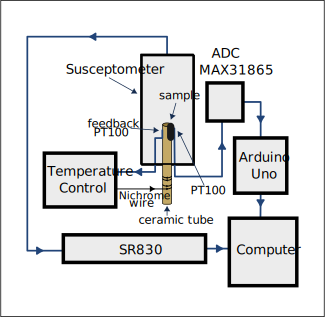
\includegraphics[width= \linewidth]{setup.png}
  \caption{Final setup would look like this with temperature and susceptibility data}
  \label{fig:setupimage}
\end{figure}

\section{Results and Conclusion}

We have made an AC susceptometer for measuring magnetic properties of material. These instruments can measure magnetic susceptibility automatically of a sample and with extended instrumentation as we talked in Experimental setup is capable of measuring magnetic properties in temperature sweeps. This can help tremendously in finding magnetic phase transition. We didn’t find that here but we find magnetic susceptibility of some of the samples. For example we found magnetic Susceptibility of LSMO ($La_{0.7}Sr_{0.3}MnO_3$) at frequency 1kHz, at room temperature is $0.01227 m^3/mol$ with reference to nickel's susceptibility taken at $0.004423 m^3/mol$\cite{PhysRev.17.678}. Here, calibration constant is $\alpha \approx 7485$ (Look equation \ref{thiseq} to make sense).


%% \setlength{\bibsep}{0pt plus 0.3ex}
\addcontentsline{toc}{section}{References}
\bibliographystyle{plainnat}
\bibliography{documentation}



\end{document}


